\documentclass[10pt,t]{beamer}
\usepackage{graphicx}
\usepackage{color}
\definecolor{myblue}{rgb}{.8, .8, 1}
\usepackage{amsmath}
\usepackage{empheq}
\usepackage[varg]{txfonts}   
\usepackage{float}
\usepackage{fancyhdr}
\usepackage{slashed}
\usepackage[skins,theorems]{tcolorbox}
\tcbset{highlight math style={enhanced,
  colframe=red,colback=white,arc=0pt,boxrule=1pt}}
\newcommand{\highlight}[1]{%
\colorbox{blue!10!white}{$\displaystyle#1$}}




\usetheme{Copenhagen}
\title{Studying Higgs production at the LHC and future colliders}
\subtitle{\small LIP summer internship}
\author{\textbf{Sebastião Fonseca}}
\institute{Project supervisor: João Pires } 
\date{08/09/2023}

\titlegraphic{
\includegraphics[width=0.3\textwidth]{LIP.png}}
\begin{document}

\frame{\titlepage}


\begin{frame}{Gauge Symmetries}
    
    
    \pause
    \small
    \center Example: $U(1)$ gauge symmetry on a Dirac field
    \begin{columns}
    \begin{column}{0.5\textwidth}
       \begin{equation*}
        \mathcal{L} = \bar{\Psi}\left(i\gamma^{\mu}\partial_{\mu}-m\right)\Psi
       \end{equation*}      
    \end{column}
    \begin{column}{0.5\textwidth}
       \begin{equation*}
         \Psi(x)\rightarrow e^{-i\alpha(x)}\Psi(x)
       \end{equation*}    
    \end{column}
    \end{columns}
    
    \pause
    
    \begin{equation*}
       \implies \mathcal{L}´ = \bar{\Psi}\left(i\gamma^{\mu}\partial_{\mu}-m\right)\Psi+\bar{\Psi}\gamma^{\mu}\left(\partial_{\mu}\alpha\right)\Psi
    \end{equation*}
    \small
    
    \center We have to redefine $\partial_{\mu} \rightarrow D_{\mu} $, with $D_{\mu}\Psi \rightarrow e^{-i\alpha(x)}D_{\mu}\Psi(x)$
    \pause
    \begin{columns}
    \begin{column}{0.5\textwidth}
       \begin{equation*}
        D_{\mu}\Psi = \left[\partial_{\mu}+igB_{\mu} \right]\Psi
       \end{equation*}      
    \end{column}
    \begin{column}{0.5\textwidth}
       \begin{equation*}
         B^{\mu} \rightarrow B^{\mu} + \frac{\partial^{\mu}\alpha(x)}{g}
       \end{equation*}    
    \end{column}
    \end{columns}

    \pause

    \begin{equation*}
        \tcbhighmath[boxrule=2pt,arc=1pt,colback=blue!10!white,colframe=blue]{\mathcal{L} = i\bar{\Psi}\gamma^{\mu}\partial_{\mu}\Psi -m\bar{\Psi}\Psi-\frac{1}{4}F^{\mu\nu}F_{\mu\nu}-gB_{\mu}\gamma^{\mu}\bar{\Psi}\Psi}
    \end{equation*}

    \pause

   \center But mass terms for the fields, such as $m^2B_{\mu}B^{\mu}$, break gauge symmetry.
    \begin{equation*}
         m^2B^{\mu}B_{\mu} \rightarrow  m^2B^{\mu}B_{\mu} + \frac{2}{g}B^{\mu}\partial_{\mu}\alpha(x)+\frac{1}{g^2}\partial^{\mu}\alpha(x)\partial_{\mu}\alpha(x)
    \end{equation*}

    
\end{frame}


\begin{frame}{Spontaneous Symmetry Breaking (SSB)}
    
    \begin{equation*}
    \mathcal{L} = \frac{1}{2}\left(\partial^{\mu}\phi\right)\left(\partial_{\mu}\phi\right)-V(\phi) \quad\text{;}\quad  V(\phi)=\frac{1}{2}\mu^2\phi^2+\frac{1}{4}\lambda\phi^4
    \end{equation*}
    
    
    
    \begin{columns}[T]
        \begin{column}{0.5\textwidth}
        \centering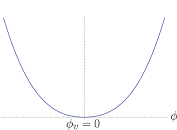
\includegraphics[width=0.7\textwidth]{Images/SSB.png}
        \small \center $\mu^2>0$
        \end{column}

        \begin{column}{0.5\textwidth}
        \centering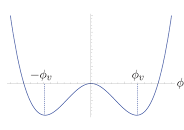
\includegraphics[width=0.7\textwidth]{Images/SSB2.png}
        \small \center $\mu^2<0$
        \end{column}
        
    \end{columns}
    
    \pause
    
    \begin{equation*}
       \small \phi(x) = v+h(x) \implies \mathcal{L} = \frac{1}{2}\left(\partial^{\mu}h\right)\left(\partial_{\mu}h\right)- \highlight{\frac{1}{2}\left(2\lambda v^2\right)h^2}-\lambda v h^3-\frac{1}{4}\lambda h^4+\frac{1}{4}\lambda v^4,
    \end{equation*}

    \small The $h(x)$ perturbations have mass $m = \sqrt{2\lambda}v$
    

\end{frame}


\begin{frame}{The U(1) Higgs Mechanism}
    
    \begin{equation*}
    \small \mathcal{L} = \left( D^{\mu}\phi\right)^* \left( D_{\mu}\phi\right) -\mu^2|\phi|^2-\lambda|\phi|^4-\frac{1}{4}F^{\mu\nu}F_{\mu\nu}
    \end{equation*}

    \pause
    
    \center Introducing perturbations  $\phi(x) = \frac{1}{\sqrt{2}}\left(v+h(x)+i\chi(x)\right)$.
    
    \begin{equation*}
         \mathcal{L} = \frac{1}{2}\left(\partial^{\mu}\chi\right)\left(\partial_{\mu}\chi\right)+\frac{1}{2}\left(\partial^{\mu}h\right)\left(\partial_{\mu}h\right)-\lambda v^2 h^2 
          +\frac{1}{2}g^2v^2B^{\mu}B_{\mu}+gvB_{\mu}\partial^{\mu}\chi + (...)
    \end{equation*}

    \pause
    
     \center Performing the gauge transformation $B_{\mu}= B_{\mu}+\frac{1}{gv}\partial_{\mu}\chi$.

    \begin{equation*}
         \mathcal{L} = \frac{1}{2}\left(\partial^{\mu}h\right)\left(\partial_{\mu}h\right)-\lambda v^2 h^2 
        +\highlight{\frac{1}{2}g^2v^2B^{\mu}B_{\mu}}+(...)
    \end{equation*}

    \center The $B $ field now has mass $m_B = gv$.
    
\end{frame}


\begin{frame}{Higgs Production Processes}
    \small
    There are four main production processes for the higgs: gluon fusion, top anti-top fusion, vector boson fusion, and vector boson \textit{bremsstrahlung}.
    
    Of these, gluon fusion (ggF) is by far the most important, and it will be the focus of this project
   
    \centering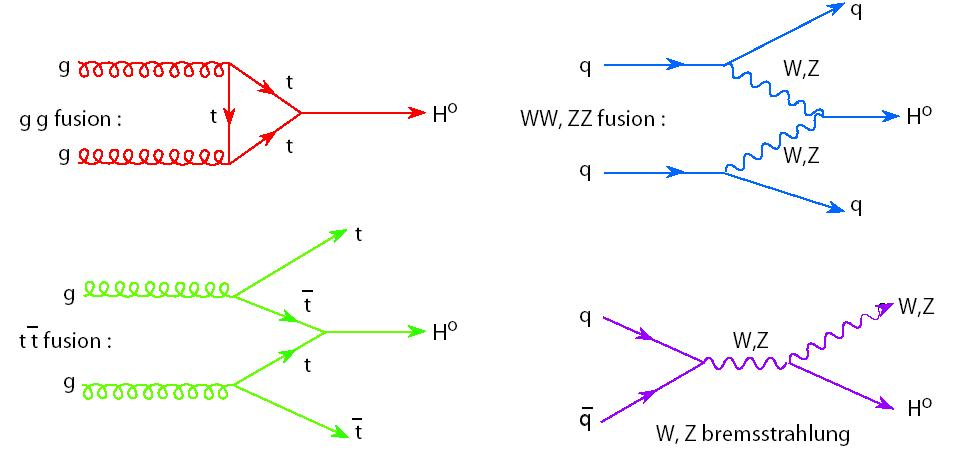
\includegraphics[width=0.8\textwidth]{Images/Higgs_prod_graphs_new2.jpg}
     
\end{frame}


\begin{frame}{Gluon Fusion at LO}

    \item \small There are two Feynman diagrams at leading order, both with the same amplitude
    \centering 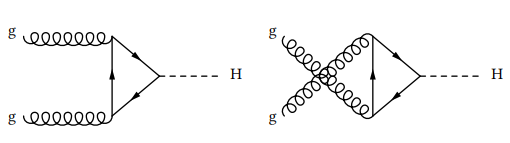
\includegraphics[width=.8\textwidth]{Images/diagram.png}
    \pause
    \scriptsize
    \begin{equation*}
        \mathcal{M} = -i\int \frac{d^4q}{(2\pi)^4} \varepsilon_1^{\mu}\left( ig_s\gamma_{\mu}T^a_{jk} \right)i\frac{(\slashed{q}+\slashed{k}_1+m)}{(q+k_1)^2-m^2}\left( -ig_s\gamma_{\nu}T^b_{kl} \right)\varepsilon_2^{\nu} 
        i\frac{(\slashed{q}+\slashed{k_1}+\slashed{k_2}+m)}{(q+k_1+k_2)^2-m^2}\left(-i\frac{g}{2}\frac{m}{m_W}\right)i\frac{(\slashed{q}+m)}{q^2-m^2}\delta^{jl}
    \end{equation*}
    
    \pause
    \normalsize
    \begin{equation*}
        \mathcal{M} = \frac{1}{4\pi}\left(\sqrt{2}G_F\right)^{\frac{1}{2}}m\alpha_sTr\left(T^aT^b\right)\highlight{\varepsilon_1^{\mu}\varepsilon_2^{\nu}\int \frac{d^4q}{i\pi^2}\frac{T_{\mu\nu}}{D_0D_1D_2}}
    \end{equation*}
    \pause
    \begin{equation*}
        T_{\mu\nu} = \mathrm{Tr}\left[(\slashed{q}+m)\gamma_{\mu}(\slashed{q}+\slashed{k}_1+m)\gamma_{\nu}(\slashed{q}+\slashed{k_1}+\slashed{k_2}+m)\right]
    \end{equation*}
    
\end{frame}


\begin{frame}{Gluon Fusion at LO (cont.)}
\small Since gluons are massless, they only have transversal components, and we can introduce the transverse projector,  $P_{T\mu\nu} = \eta_{\mu\nu} - \frac{k_{1\mu}k_{2\nu}}{k_1.k_2}$, without losing any information.

\begin{equation*}
    \implies \varepsilon_1^{\mu}\varepsilon_2^{\nu} F P_{T\mu\nu} \quad\text{, with }\quad F = \frac{1}{4}P_T^{\mu\nu}\int \frac{d^4q}{i\pi^2}\frac{T_{\mu\nu}}{D_0D_1D_2}.
\end{equation*}

\pause
Now square the amplitude and sum over all the initial states of the gluons.

\begin{equation*}
    |\overline{\mathcal{M}}|^2 = \frac{1}{2.2.8.8}\frac{1}{16\pi^2}\alpha_S^2\left(\sqrt{2}G_F\right)m^2\highlight{\sum_{pol.}\sum_{a,b=1}^8 \left|\frac{\delta^{ab}}{2}\varepsilon_1^{\mu}\varepsilon_2^{\nu} F P_{T\mu\nu}\right|^2}
\end{equation*}


\begin{equation*}
    \sum_{a=1}^8\left(\frac{P_{T\mu\nu}\eta^{\mu\alpha}\eta^{\nu\beta}P_{T\alpha\beta}}{4}F^2\right)=8\left(\frac{P_T^{\mu\nu}P_{T\mu\nu}}{4}F^2\right) = 4F^2 
\end{equation*}

\pause
So the expression for total amplitude squared is

\begin{equation*}
    \implies |\overline{\mathcal{M}}|^2  = \frac{\sqrt{2}G_F\alpha_S^2}{32^2\pi^2}m^2F^2
\end{equation*}

\end{frame}


\begin{frame}{Result for the Amplitude}
    \small
    \begin{equation*}
        {F = 2m + m\left(4m^2-m_H^2\right)C_0\left(k_1,k_2,m\right)}
    \end{equation*}

    \begin{equation*}
         C_0(k_1,k_2,m) = \begin{cases}
            -\frac{2}{m_H^2}\arcsin^2{\left(\sqrt{\frac{1}{\rho}} \right)}  ,& \rho= \frac{4m^2}{m_H^2} > 1  \\
             \frac{1}{m_H^2}\left(\log\left( \frac{1+\sqrt{1-\rho}}{1-\sqrt{1-\rho}}\right)-i\pi \right)^2,& \rho= \frac{4m^2}{m_H^2} < 1
             \end{cases}
     \end{equation*}

    \vspace{2mm}
    \pause

    
    \begin{equation*}
     \tcbhighmath[boxrule=2pt,arc=1pt,colback=blue!10!white,colframe=blue]{|\overline{\mathcal{M}}|^2 = \frac{\sqrt{2}G_F\alpha_S^2m_H^4}{64^2\pi^2}A\left(\rho\right)}
    \end{equation*}

    with 

    \begin{equation*}
    A\left(\rho\right) = \begin{cases}
    
            \rho^2\left( 1+(1-\rho)\arcsin^2{\left(\sqrt{\frac{1}{\rho}} \right)}\right)^2  ,& \rho > 1  \\
            
            \rho^2\left( 1-\frac{1}{4}(1-\rho)\left| \log\left( \frac{1+\sqrt{1-\rho}}{1-\sqrt{1-\rho}}\right)-i\pi \right|^2\right)^2,& \rho  < 1 .
            \end{cases}
    \end{equation*}
    
\end{frame}


\begin{frame}{Amplitude Plot}
\small
\begin{figure}[ht]
    \centering
    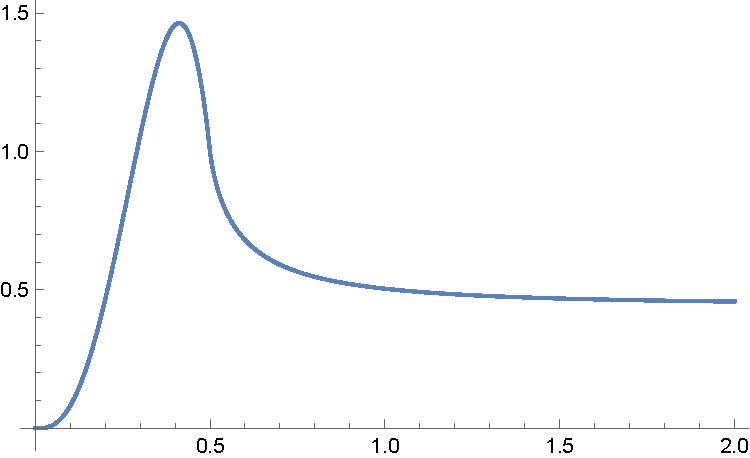
\includegraphics[width=.6\textwidth]{Images/f(p).pdf}
    \caption{Plot of $A\left(\rho\right)$ for quark masses from $0$ to $2m_H$ }
 
\end{figure}
    \vspace{5mm}
    \begin{equation*}
         |\overline{\mathcal{M}^t}|^2 \simeq 150 |\overline{\mathcal{M}^b}|^2
     \end{equation*}



\end{frame}


\begin{frame}{Cross Section at LO}
     \begin{equation*}
         \mathcal{M}_{total} =  \sum_{quarks} \mathcal{M}^q \implies |\overline{\mathcal{M}_{total}}|^2 \simeq |\overline{2\mathcal{M}^t}|^2= 4|\overline{\mathcal{M}^t}|^2
    \end{equation*}

        \begin{equation*}
             |\overline{\mathcal{M}_{total}}|^2=\frac{\sqrt{2}G_F\alpha_S^2m_H^4}{32^2\pi^2}\rho^2\left( 1+(1-\rho)\arcsin^2{\left(\sqrt{\frac{1}{\rho}} \right)}\right)^2 
        \end{equation*}

        \pause
     

       The cross section is
       \begin{equation*}
           \sigma_{part} =\frac{1}{2s} \int \frac{d^3p}{(2\pi)^32p_0}(2\pi)^4 |\overline{\mathcal{M}_{total}}|^2 = \highlight{\frac{\pi}{m_H^2}\delta\left(s-m_H^2\right)|\overline{\mathcal{M}_{total}}|^2}
       \end{equation*}
       
       \pause
       \begin{equation*}
            \sigma_{total} = \frac{\sqrt{2}G_F\alpha_S^2m_H^2}{32^2\pi S}A\left(\rho\right) \int dy~ f\left(\sqrt{\frac{m_H^2}{S}}\exp(y)\right)f\left(\sqrt{\frac{m_H^2}{S}}\exp(-y)\right)
        \end{equation*}
       
\end{frame}


\begin{frame}{Computational Results}
    \center  Ihixs 2 - configuration
            
            $m_H = 125 $GeV, $\mu_R = 62.5$ GeV, $\mu_F = 62.5$ GeV
            \small
    \begin{columns}
        \begin{column}{0.5\textwidth}
          \begin{figure}
                \centering
                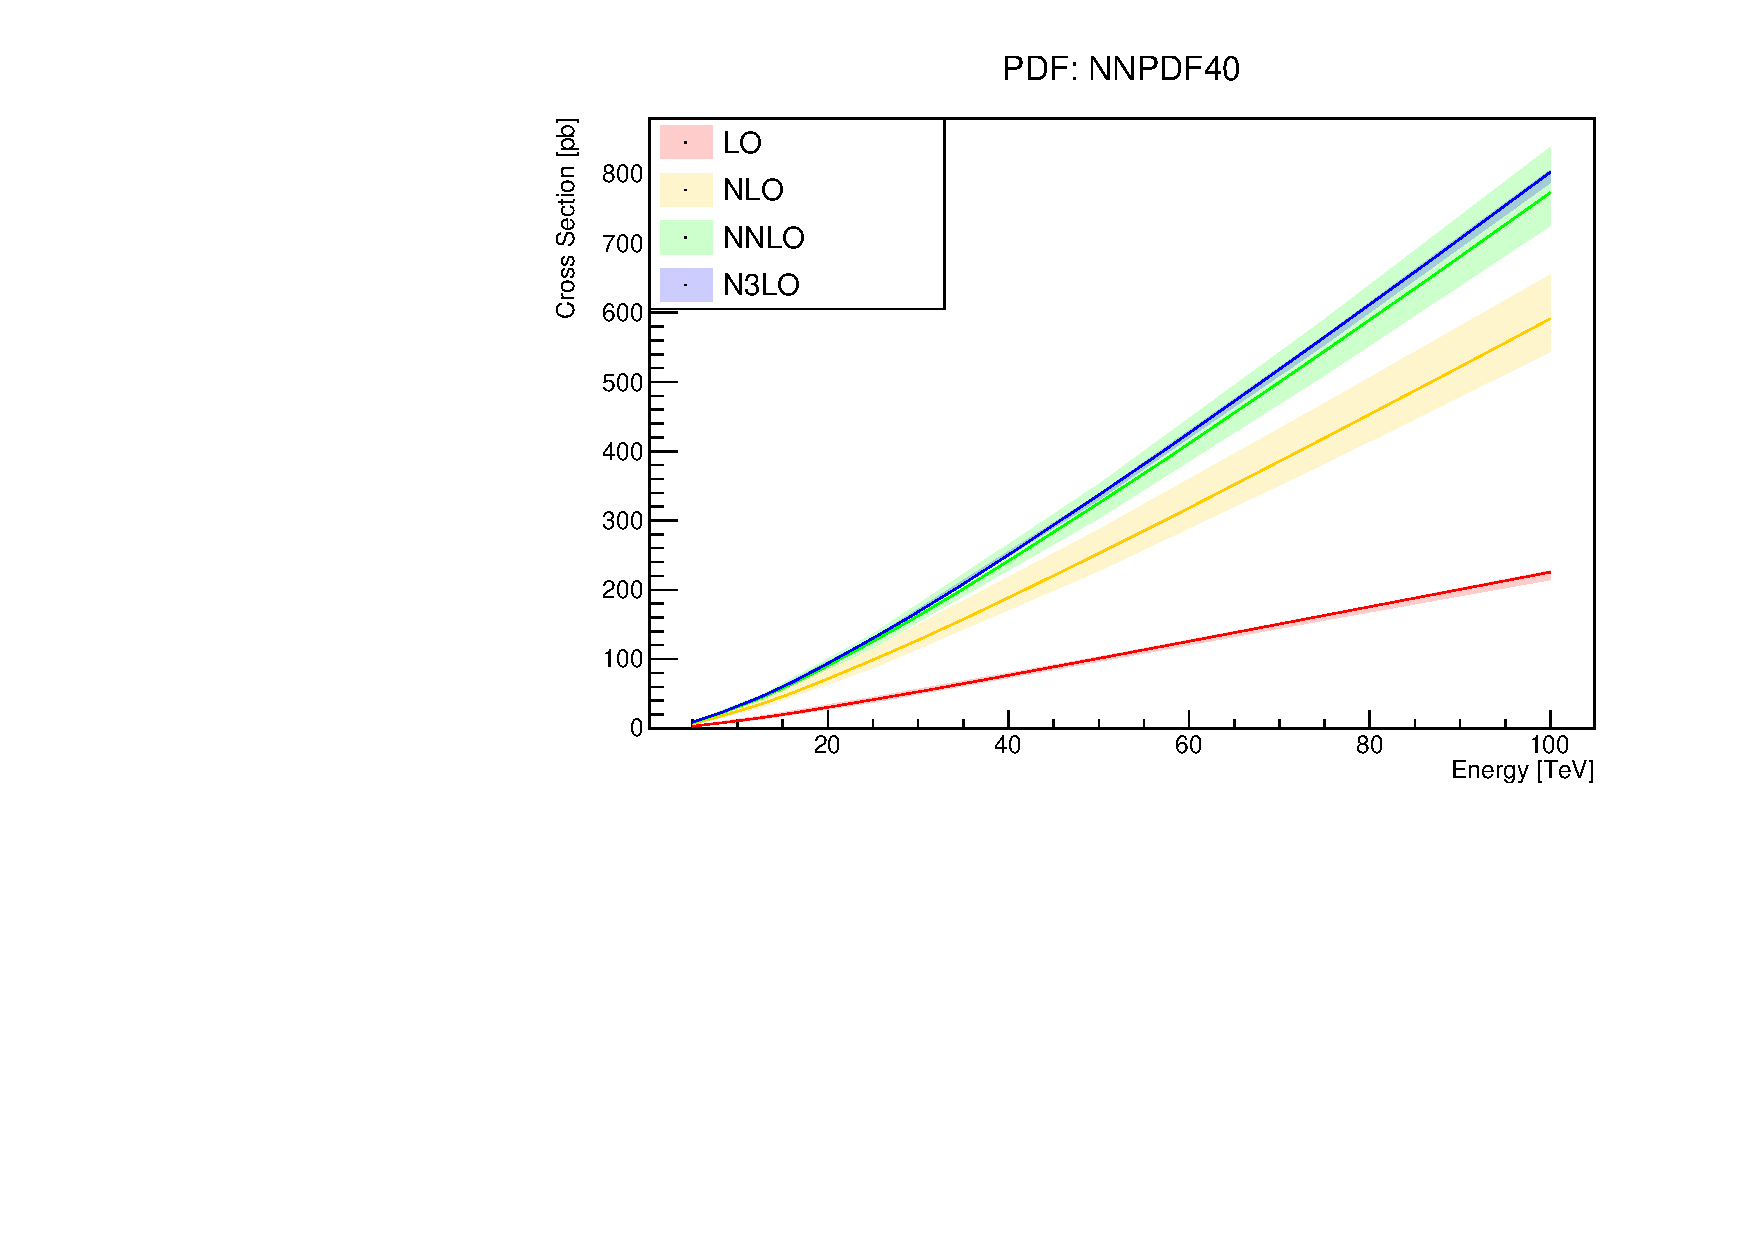
\includegraphics[scale=0.3]{Images/NNPDF40_XS.pdf}
                 \caption{ Plot of the cross section as a function of the collision energy}
           \end{figure}
            
        \end{column}


        
        \begin{column}{0.5\textwidth}
            

            \begin{figure}
                 \centering
                 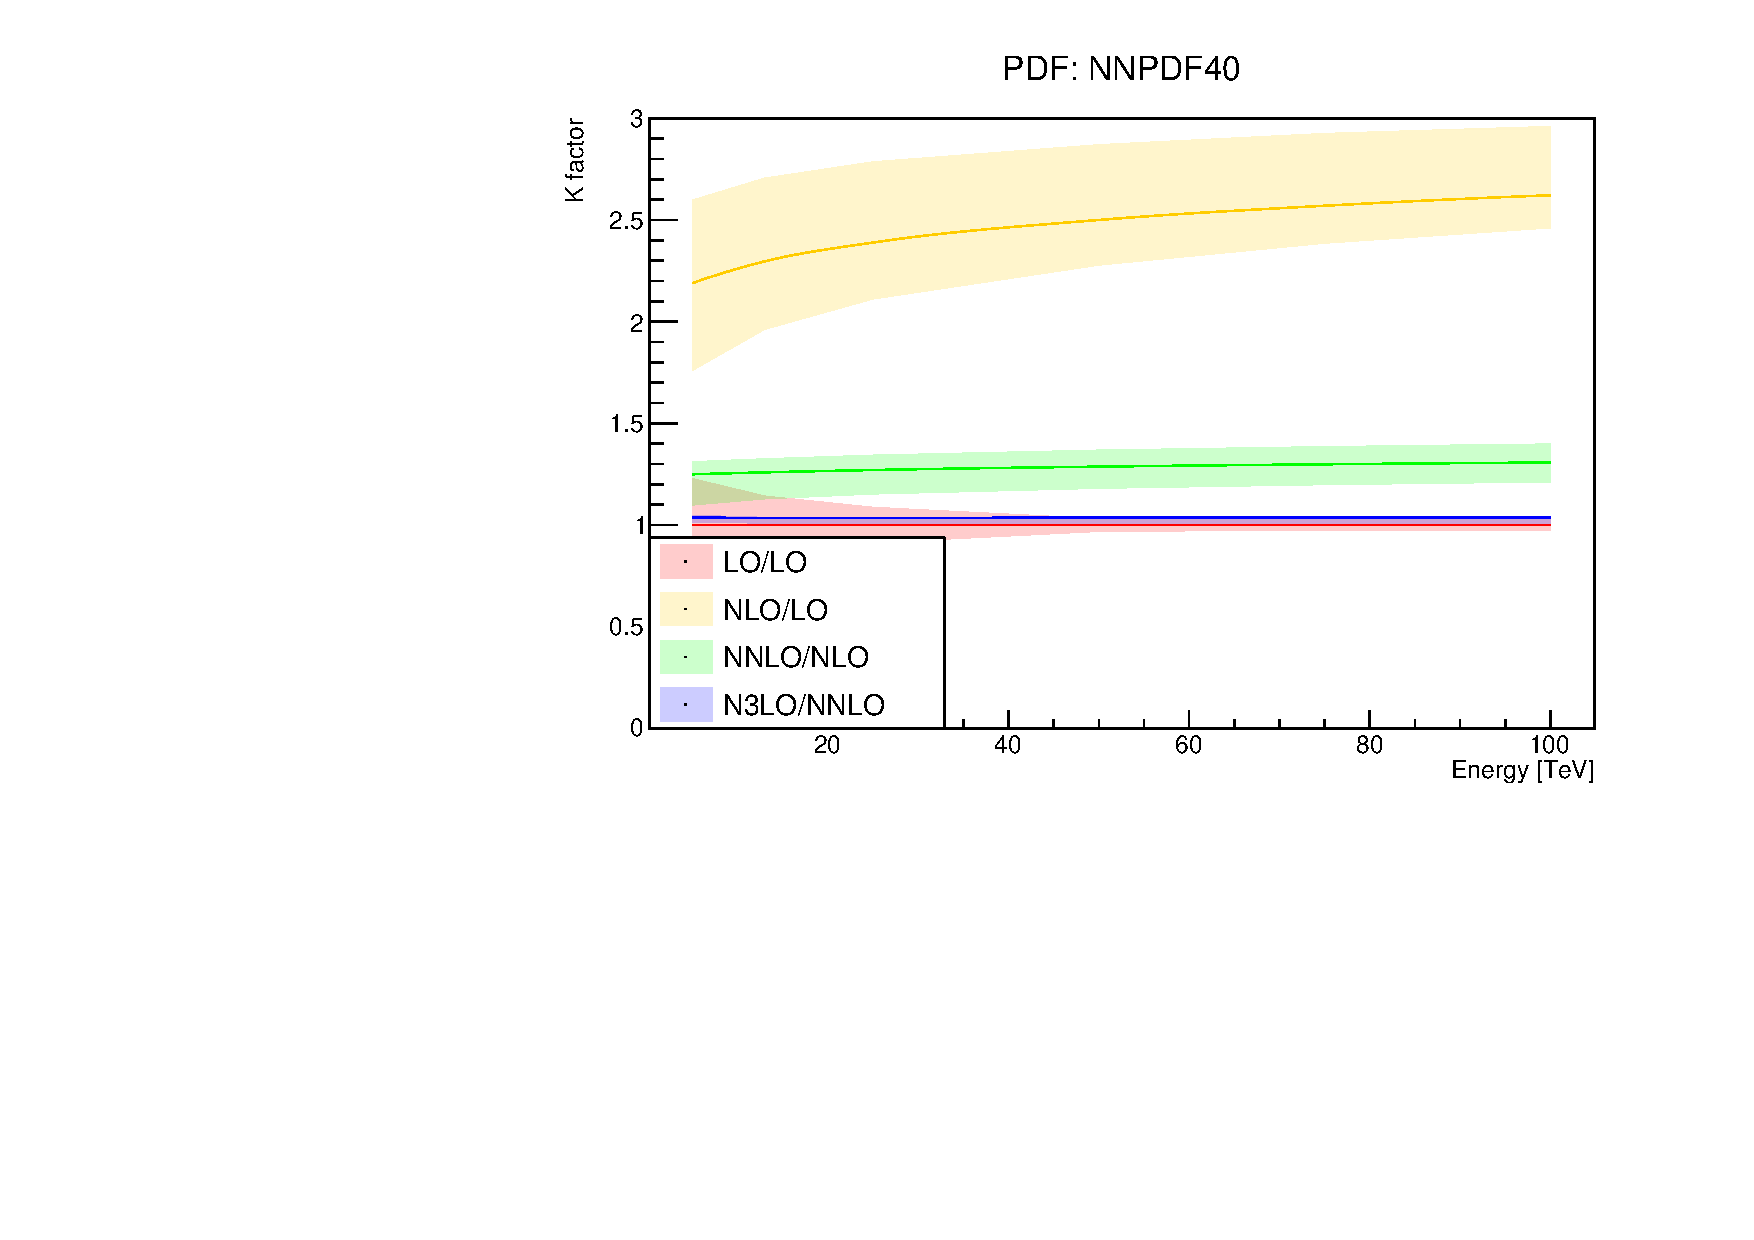
\includegraphics[scale=0.3]{Images/NNPDF40_K.pdf}
                 \caption{ Plot of the relative contributions of each order as a function of the collision energy}
            \end{figure}
            
        \end{column}
        
    \end{columns}
\end{frame}


\begin{frame}{Computational Results (cont.)}

     \hspace{2mm}   
     \small
    \begin{columns}
        \begin{column}{0.5\textwidth}
          \begin{figure}
                \centering
                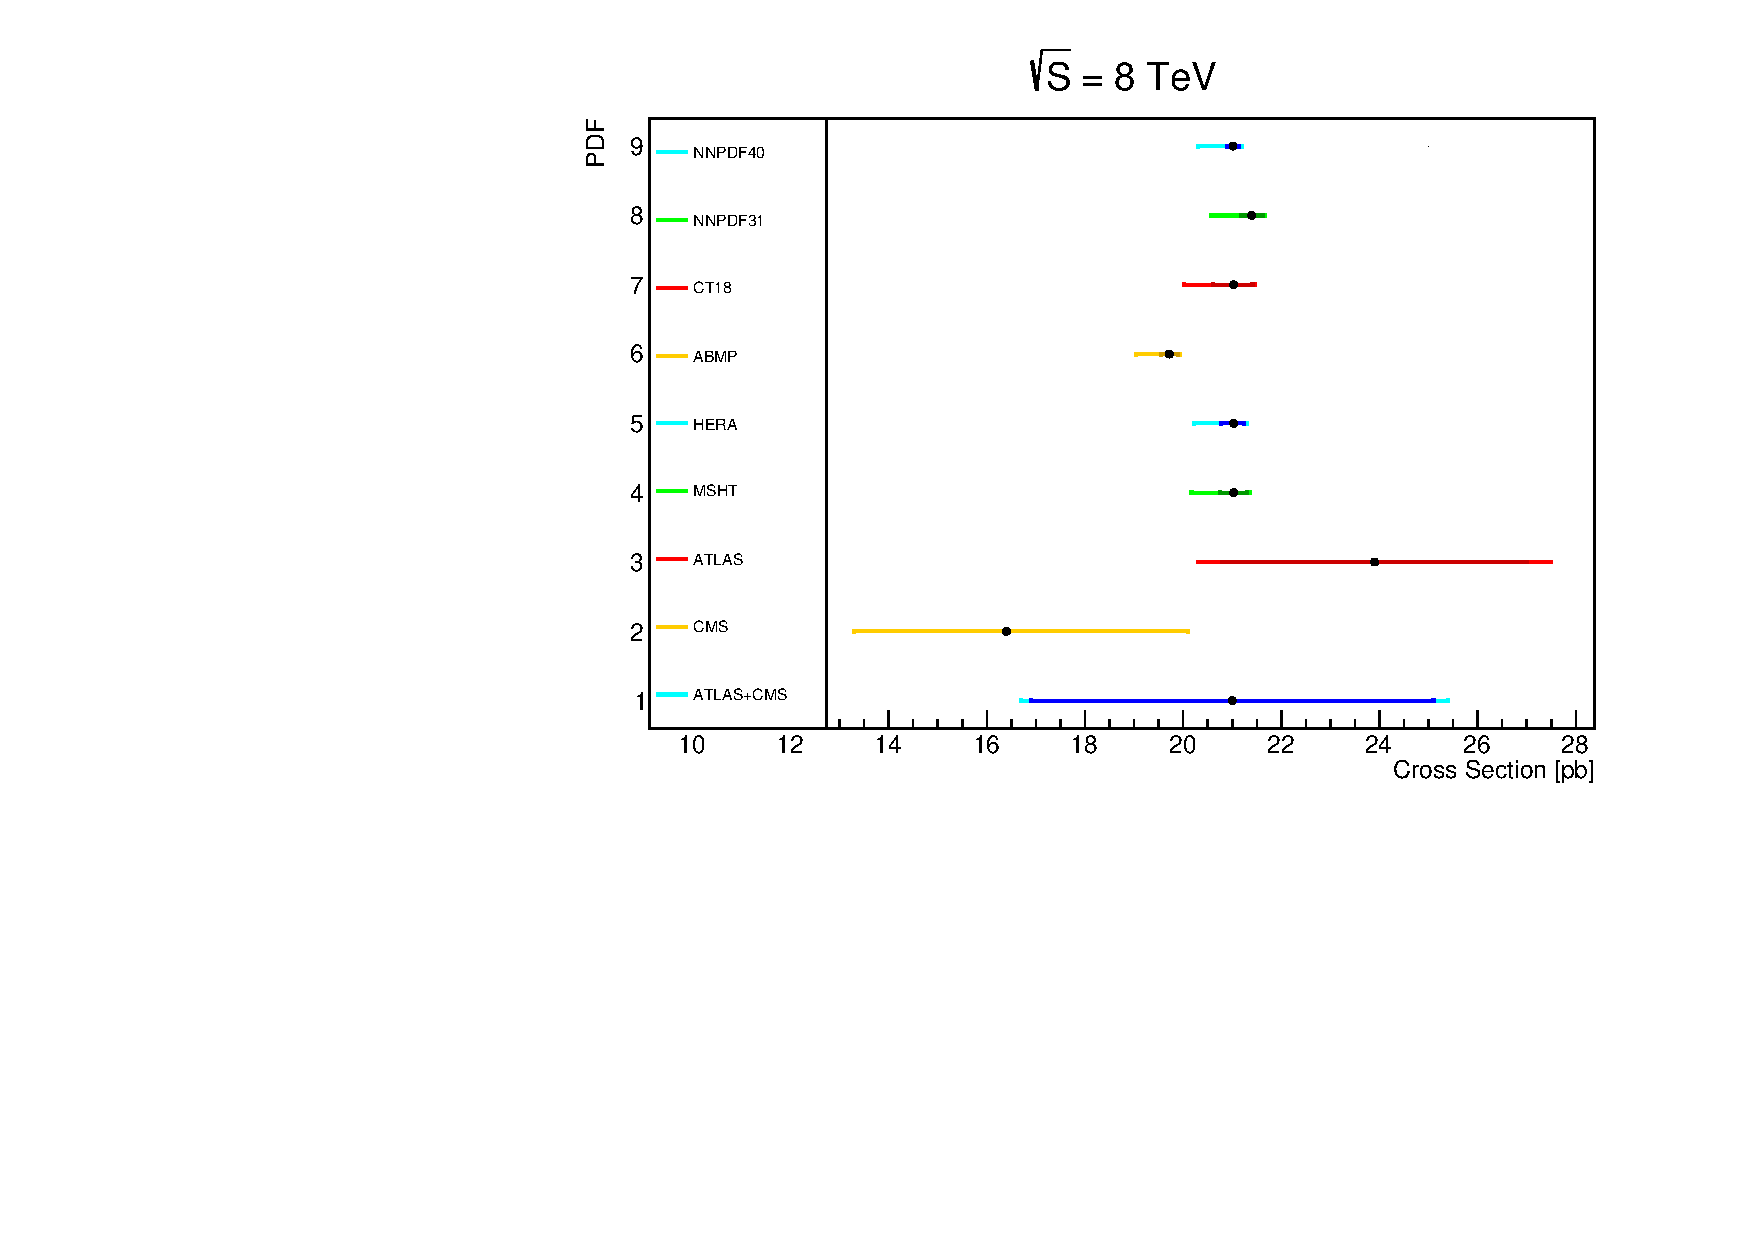
\includegraphics[scale=0.3]{Images/Graph2.pdf}
                 \caption{Plot of the cross section result for various PDFs at 8 TeV}
           \end{figure}
            
        \end{column}


        
        \begin{column}{0.5\textwidth}
            

            \begin{figure}
                 \centering
                 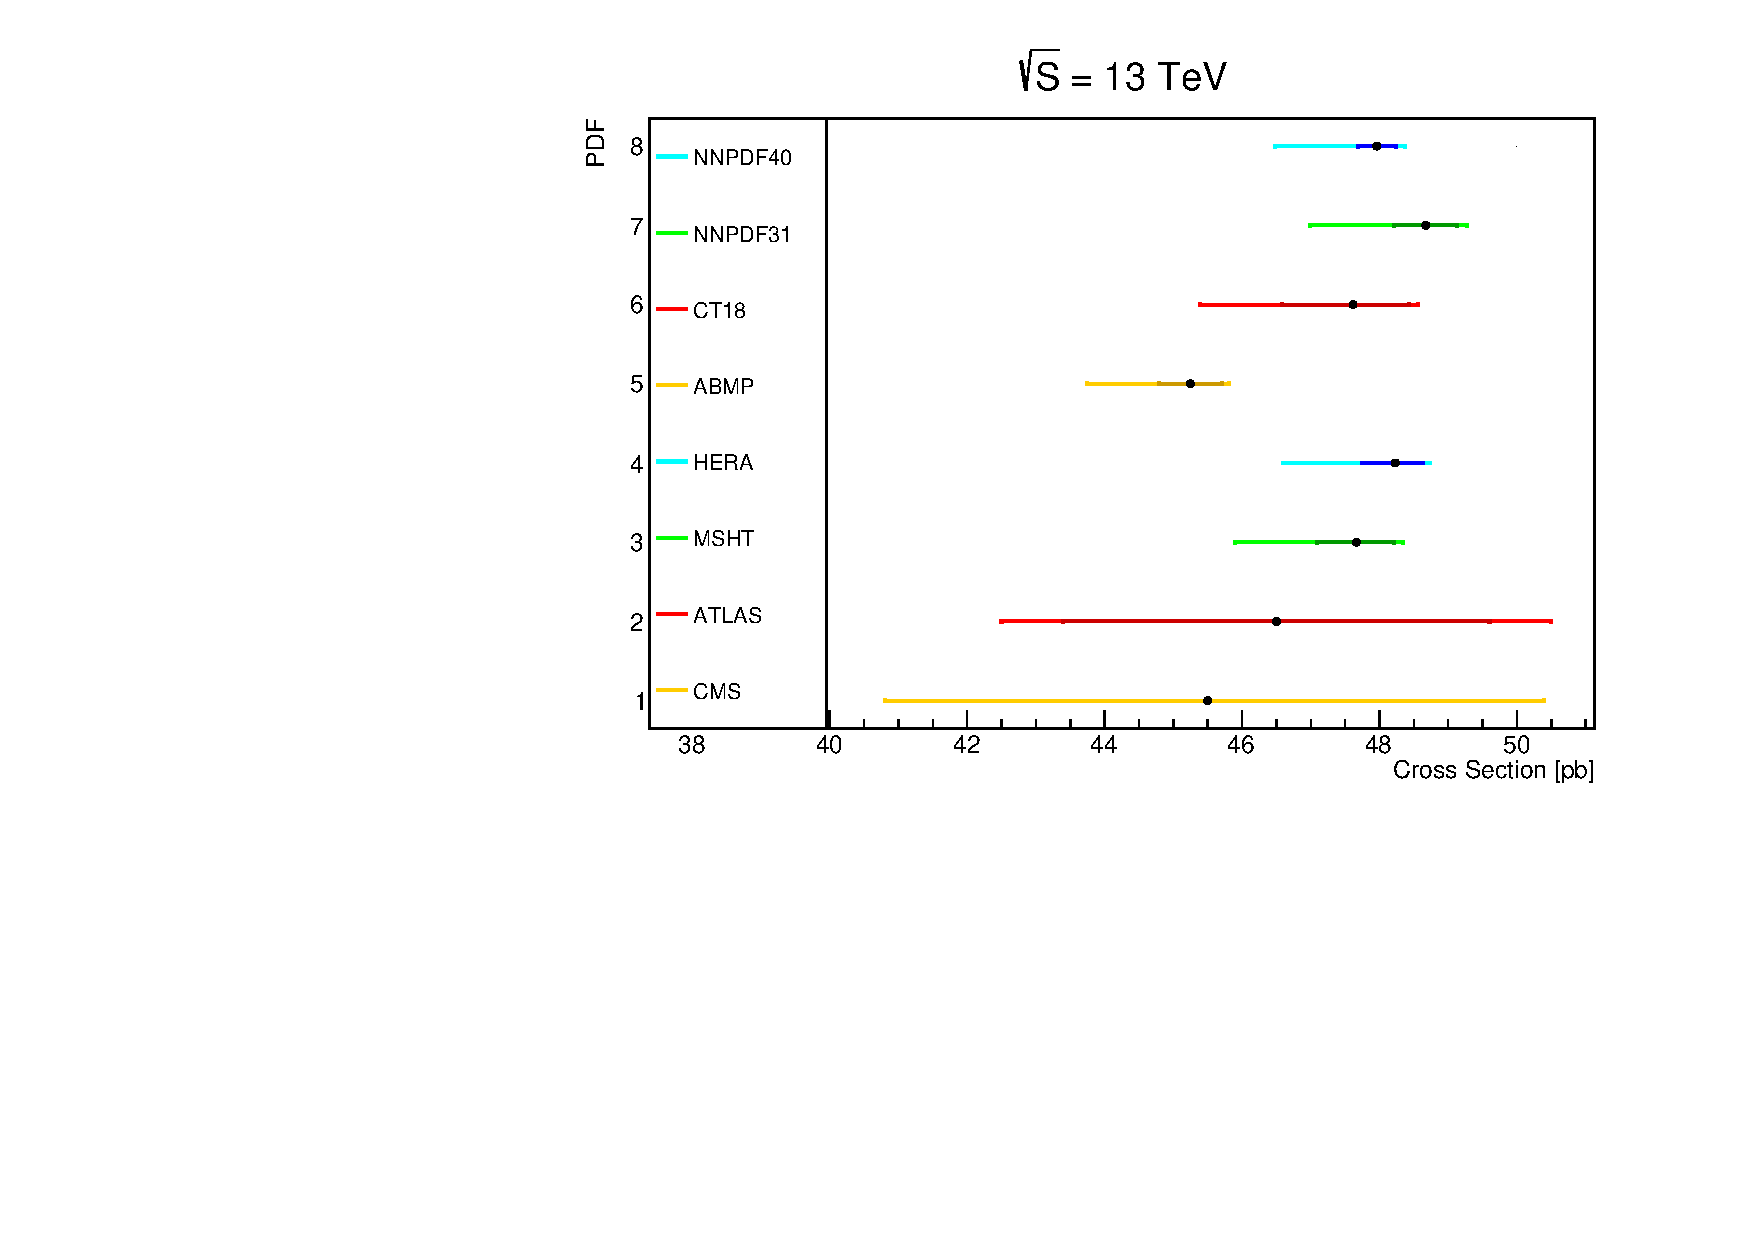
\includegraphics[scale=0.3]{Images/Graph3.pdf}
                 \caption{Plot of the cross section result for various PDFs at 13 TeV}
            \end{figure}
            
        \end{column}
        
    \end{columns}
\end{frame}


\begin{frame}{Conclusions}
     
     \begin{equation*}
         N_{H\rightarrow\gamma\gamma} = BR_{H\rightarrow\gamma\gamma} \times\left[\sigma_{7TeV} \times 4.8fb^{-1} + \sigma_{8TeV} \times 20.7fb^-1\right] \approx 1000
     \end{equation*}
    
     \begin{figure}
                \centering
                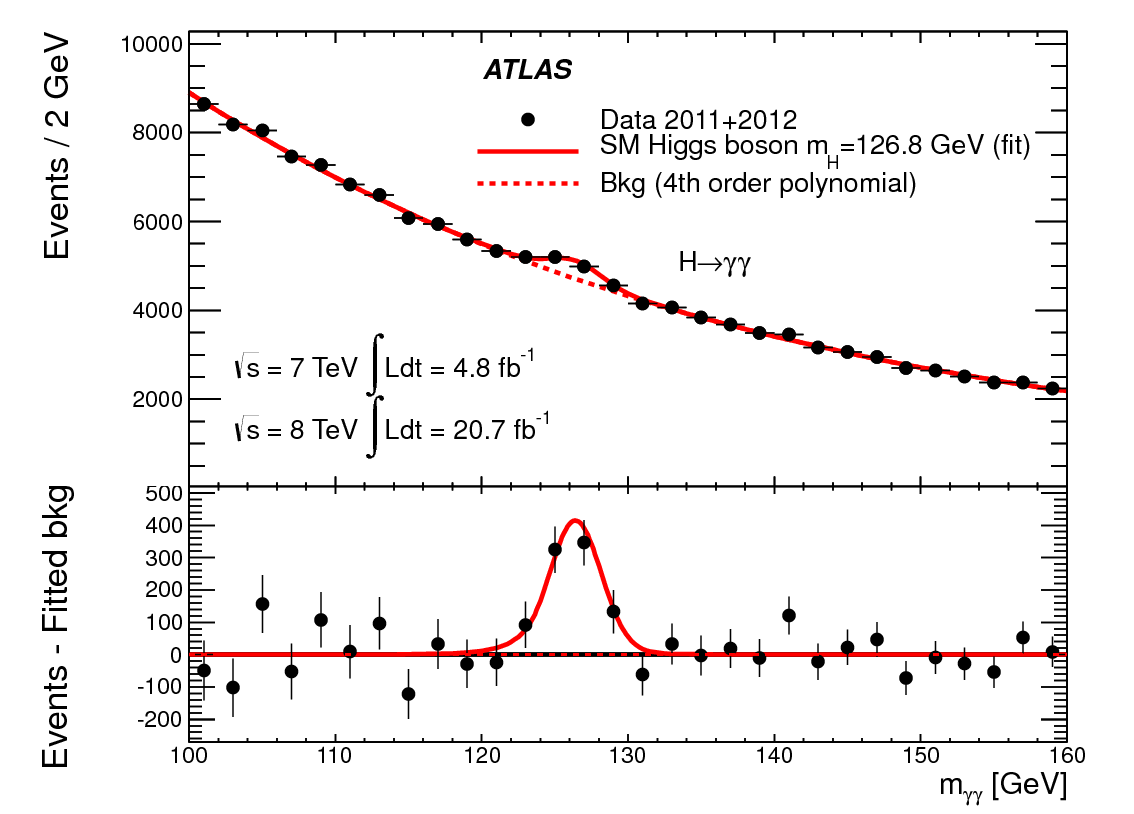
\includegraphics[scale=0.15]{Images/Discovery.jpg}
                 
     \end{figure}
    \pause

    \center Future Circular Collider (FCC)
     \begin{equation*}
         N_{H\rightarrow\gamma\gamma} = BR_{H\rightarrow\gamma\gamma} \times\left[\sigma_{100TeV} \times (0.2-2)ab^{-1}\right] \approx (0.32-3.2) \times 10^6 \text{ per year!}
     \end{equation*}
     

\end{frame}




\begin{frame}{Acknowledgements}
    \vspace{3cm}
    \centering \Huge Thank you!
\end{frame}




\end{document}